%-----------------------------------------------------------------------
% 
%-----------------------------------------------------------------------
%
%     
%
%
%%%%%%%%%%%%%%%%%%%%%%%%%%%%%%%%%%%%%%%%%%%%%%%%%%%%%%%%%%%%%%%%%%%%%%%%


\documentclass[twoside]{article}
\usepackage{amsmath,amsthm,amssymb,verbatim}

%     If your article includes graphics, uncomment this command.
\usepackage{graphicx}

%     If the article includes commutative diagrams, ...
%\usepackage[cmtip,all]{xy}

\usepackage{url}

\usepackage{fancyhdr}
\pagestyle{fancy}

\def\blfootnote{\xdef\@thefnmark{}\@footnotetext} 
\long\def\symbolfootnote[#1]#2{\begingroup%
\def\thefootnote{\fnsymbol{footnote}}\footnote[#1]{#2}\endgroup} 

	\addtolength{\oddsidemargin}{1cm}
	\addtolength{\evensidemargin}{-1cm}

\setcounter{page}{1}

\begin{document}

%     If you need symbols beyond the basic set, uncomment this command.
%\usepackage{amssymb}


\newtheorem{theorem}{Theorem}[section]
\newtheorem{lemma}[theorem]{Lemma}

\theoremstyle{definition}
\newtheorem{definition}[theorem]{Definition}
\newtheorem{example}[theorem]{Example}
\newtheorem{xca}[theorem]{Exercise}

\theoremstyle{remark}
\newtheorem{remark}[theorem]{Remark}

\numberwithin{equation}{section}


\date{}
\lhead[]{}
\chead[\underline{Deep Learning for Riemann Zeta}]{\it{O. Shanker}}
\rhead[]{}

% \title[short text for running head]{full title}
\title{\bf{Deep Learning for Riemann Zeta Function: Large Values and Karatsuba problem}}

\maketitle


%    author one information
% \author[short version for running head]{name for top of paper}
\author{{\textbf{O. Shanker}},}
\thanks{ Mountain View, CA 94041, U. S. A. email: oshanker@gmail.com}

\thispagestyle{fancy}

%    Abstract is required.
\begin{abstract}
The study of large values of the Riemann zeta function on the critical axis is a topic of mathematical
interest.  One such mathematical topic is the Karatsuba problem. It will be useful to have empirical results on the distribution of large values of the zeta function, to give insights 
into the theoretical studies.  Since evaluating the Riemann zeta function at large heights  is a non-trivial task, requiring much computer time 
(and some knowledge of special techniques to find the roots), we apply
machine learning to the problem.

\end{abstract}
{\textbf {Keywords}:} Circular Unitary Ensemble, Riemann zeta, Value Distribution,  Large Values 
{\textbf {Mathematics Subject Classification (MSC)}:} 11M06, 11-04.


\symbolfootnote[0]{*}


\section{Introduction}

 There have been many applications of machine learning in mathematics, including 
the application of Neural networks to the Riemann zeta function~\cite{osneural}.
Deep Learning has been applied to study the Goldbach partition function~\cite{kim2022}.
Here we study its use to provide insights into  the Karatsuba problem~\cite{K5, Kor1}.


\section{\label{sec2}Materials and Methods}

\begin{figure*}
\centering
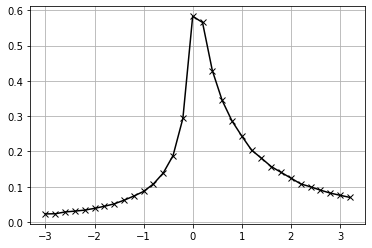
\includegraphics[width=0.8\textwidth]{1.png}
\caption[]{ 
  Distribution of $\zeta_{max}$. 
  }
\vspace{1mm}
\label{z1}
\end{figure*}

\subsection{\label{seckaratsuba}Karatsuba Problem}

Among the many studies of large values of the Riemann zeta function on the critical axis, Karatsuba~\cite{K5} studied 
\begin{equation}
F(T; H)  \, = \, max_{|t-T| \le H} \zeta ( 0.5+it ) 
\label{eqRie}
\end{equation}
where $H$ is small compared to $T$. The ramifications of the Karatsuba problem are explained and
reviewed in, e.g.,  Korolov~\cite{Kor1}.  

The freezing transition scenario occurs in the statistical mechanics of 1/f-noise random energy models. Ref~\cite{FK} argue that it  also governs the value distribution of the maximum of the modulus of the characteristic polynomials  of large N × N (circular unitary ensemble, CUE) random unitary  matrices for large N.  Given the relation of CUE matrices to the Riemann zeta function~\cite{oscue}, the arguments have implications to the topic we are studying. Other works studying large values of the Riemann zeta function over short intervals are \cite{Feng, Tihanyi, FTH, Ivic}. Fig.~\ref{z1} gives the distribution of $max_{|t-T| \le H}| \zeta ( 0.5+it ) |$ for $T=10^{12}, H=26*gram~interval$.  The value of $H$ is motivated by the correspondence with the CUE. In what follows, we will denote by $\zeta_{max}$ the  $max_{|t-T| \le H}| \zeta ( 0.5+it ) |$ for this choice of $T$ and $H$.


\subsection{\label{secwhy}Why Machine Learning?}

At large heights evaluating the Riemann zeta function  is a non-trivial task, requiring much computer time 
(and some knowledge of special techniques to find the roots).  It would be useful to apply
machine learning
as a guide to identify the T values where we can expect to see the behaviour of interest.

We use TensorFlow~\cite{FrancoisChollet 2021} as the python framework to perform the machine learning 
task. We have to  decide what algorithm we should use, and what features we will use for prediction.
Regarding the feature set, 
Ref~\cite{osneural} found that the behavior of the zeta function at Gram points 
is a good starting point to extract features for use in prediction. 
Ref.~\cite{Shanker 2018a} further showed that Gram points have interesting properties 
which distinguish them from random points on the critical line. 
Related  results can be found in Ref.~\cite{os6, Shanker 2018b,Shanker 2020}. We therefore
use as our feature set for prediction the values of the rotated Riemann zeta function at the Gram points.
We then use machine learning to predict where to find the largest values of $\zeta_{max}$.

\subsection{\label{seccalc}Calculating the sample values}

We study the Riemann zeta studies  at a
height $T = 10^{12}$. We use the well-known correspondence $N \thicksim \ln(T/2\pi)$ where $N$ 
is the size of the unitary matrix we should consider for the CUE. Thus, we chose $N = 26$ for our
study.  This leads to an interval of $2\pi$ in the height $t$,  containing $N$ zeros.
We studied $500000$ gram intervals  to generate the distributions.

At large heights evaluating the Riemann zeta function  is a non-trivial task, requiring much computer time. 
We numerically evaluate $|\zeta(1/2 + it)|$ over ranges of length $2\pi$, 
 and find the maximum value $\zeta_{max}(2\pi; T )$ in each range. 
 We use the amortized complexity algorithm ~\cite{hiary}, 
 which is suitable for computing $\zeta(1/2 + it)$ at many points.

\begin{figure*}
\centering
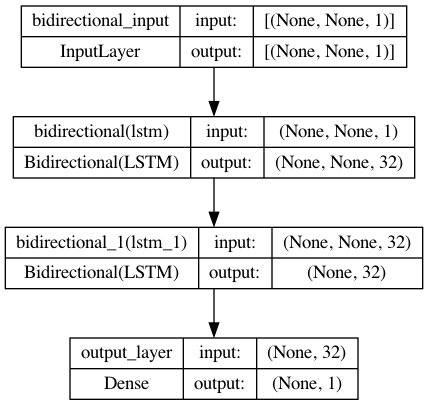
\includegraphics[width=0.8\textwidth]{2.png}
\caption[]{ 
  LSTM model. 
  }
\vspace{1mm}
\label{z2}
\end{figure*}

\begin{table}
\centering \(\begin{array}{cccccccccccc}

\hline
\hline
 Layer      &Output  &Param    \\
 (type)    &  width& count \\
\hline
\hline
layer 1            &32   &     2304     \\ 
 (Bidirectional)      &  & \     \\                                                    
\hline
layer 2            &32          &    6272      \\
 (Bidirectional)                 &  & \\                                                                                                    
 \hline
output layer   &    1          &      33        \\
 (Dense)                 &  & \\                                                                                                    
\hline
\hline
\end{array}\)
\caption{LSTM Model trainable parameters }
\label{tab:model}
\end{table}

\section{\label{sec3}Results}

\begin{figure*}
\centering
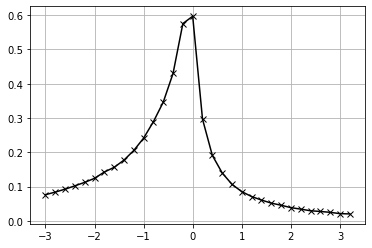
\includegraphics[width=0.8\textwidth]{3.png}
\caption[]{ 
  Training and Validation Mean Absolute Deviations.
  }
\vspace{1mm}
\label{z3}
\end{figure*}

\begin{figure*}
\centering
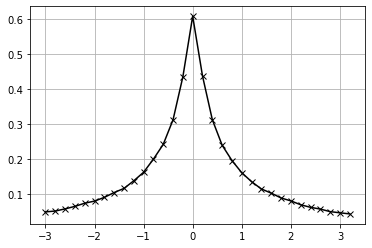
\includegraphics[width=0.8\textwidth]{4.png}
\caption[]{ 
  Comparision of model prediction with actual $\zeta_{max}$. 
  }
\vspace{1mm}
\label{z4}
\end{figure*}


\subsection{\label{sec3.1} Choosing the Model}
The data we are studying has similarities to a time series. The models of choice for
such data are Recurrent Neural Networks (RNN), in particular,  
Long Short-term Memory (LSTM)~\cite{lstm}. Further, as shown in Ref~\cite{Shanker 2018a},
the behaviour of the series looks similar whether we are moving in the forward direction 
or the backward direction. We can take advantage of this symmetry and use TensorFlow
BiDirectional layers in building the model.  
Bidirectional recurrent layers present the same information to a recurrent network in different ways, 
increasing the accuracy.
This leads to the model shown in Figure~\ref{z2} and Table~\ref{tab:model}, 
with $8609$ trainable parameters.


\begin{table}
\centering \(\begin{array}{cccccccccccc}

\hline
learning     &momentum  &epochs  \\
rate    &  &  \\
\hline
0.001 &0.895  & 15  \\
\hline
\end{array}\)
\caption{LSTM Model parameters (optimizer=tf.keras.optimizers.RMSprop)}
\label{tab:mean12}
\end{table}

\begin{table}
\centering \(\begin{array}{cccccccccccc}

\hline
training     &validation  &test \\
\hline
0.47 &0.4  & 0.43  \\
\hline
\end{array}\)
\caption{Mean Absolute Deviations}
\label{tab:mae}
\end{table}

\subsection{\label{relation}Training,  Model predictions}

What is epoch, what are different data sets.
We studied $500000$ gram intervals  to generate the distributions.
We divide this into $250000$ gram intervals for the training dataset, 
$125000$ gram intervals for the validation dataset, 
and $125000$ gram intervals for the test dataset,.
Table~\ref{tab:mean12} shows the parameters used to train the model. 
Figure~\ref{z3} shows the training Mean Absolute Deviation (also called Mean Absolute Error, MAE) 
and the validation Mean Absolute Deviation as a function of the epoch.
Table~\ref{tab:mae} shows the Mean Absolute Deviations for the different data sets.  This has
to be compared with the mean value of $\zeta_{max}$, which is $19$.  Figure~\ref{z4}
shows the model prediction versus the actual value for some points.

\section{\label{conclusions}Conclusions}

We the Riemann zeta function.

\section*{Acknowledgments and Funding Statement}

 The study was done as an independent researcher. There was no
external funding.

\section*{Ethical Compliance}

 No procedures were performed  involving human participants in the study.

\section*{Data Availability Statement}

The computer programs used during the current study are
available from the corresponding author on reasonable request.

\section*{Conflict of Interest declaration} 

The authors declare that they have no affiliations with or involvement in any organization 
or entity with any financial interest in the subject matter or materials discussed 
in this manuscript.


\bibliographystyle{amsplain}
\begin{thebibliography}{10}

\bibitem{osneural} O. Shanker, ``Neural Network prediction of Riemann zeta zeros''
{\it Advanced Modeling and Optimization}, {\bf 14}, 717-728, (2012), \url{tinyurl.com/4scve3nj}.

\bibitem{kim2022} Eunmi Kim, ``Deep learning-based approximation of Goldbach partition function''
{\it  Discrete Mathematics, Algorithms and Applications}, {\bf 14}, 2150152, (2022). 

\bibitem{K5} A. A. Karatsuba, 
``Zero multiplicity and lower bound estimates of $|\zeta(s)|$",
{\it Funct.  Approx. Comment. Math.} {\bf35}(2006), 195–207

\bibitem{Kor1} Maxim A. Korolev, 
``On large values of the Riemann zeta-function on short segments of the critical line",
{\it Acta Arithmetica} {\bf166}(2014), 349–390

\bibitem{FK} Y. V. Fyodorov and J. P. Keating,
``Freezing transition and extreme values random matrix theory, $\zeta(1/2 + it)$, and disordered landscapes",
{\it Phil. Trans. R. Soc. A} {\bf372}(2014),  20120503

\bibitem{oscue} O. Shanker, 
``Random Matrix Theory explanation for Riemann Zeta Value Distribution Symmetry''
 report,
\url{https://tinyurl.com/ywhy4jsy}, 
(2022). 

\bibitem{Feng} S. J. Feng, ``On Karatsuba conjecture and the Lindelof hypothesis'' 
{\it  Acta Arith.} {\bf 114}, 295–300,  (2004)

\bibitem{Tihanyi} Norbert Tihanyi, Attila Kovacs,  and Jozsef Kovacs, 
``Computing Extremely Large Values of the Riemann Zeta Function''
{\it  Journal of Grid Computing }, {\bf 15}, 527–534 , (2017). 

\bibitem{FTH}Yan V. Fyodorov, Ghaith A. Hiary, and Jonathan P. Keating, 
``Freezing Transition, Characteristic Polynomials of Random Matrices, and the Riemann Zeta-Function''
{\it  Phys. Rev. Lett. }, {\bf 108}, 170601 , (2012). 

\bibitem{Ivic} Aleksandar Ivić, 
``On the multiplicities of zeros of $\zeta(s)$ and its values over short intervals''
{\it  Journal of Number Theory }, {\bf 185}, 65-79 , (2018). 

\bibitem {FrancoisChollet 2021} Francois Chollet, ``Deep Learning with Python''
Manning Publications,  (2021)

\bibitem{Shanker 2018a} O. Shanker, 
``Good to Bad Gram Point Ratio For Riemann Zeta Function",
{\it Experimental Mathematics} {\bf 30}, 76-85,
\url{tinyurl.com/mwd5uwc5}(2021)

\bibitem{os6} O. Shanker, 
``Generalised Zeta Functions and Self-Similarity of Zero Distributions",
{\it J.  Phys. A} {\bf39}(2006), 13983-13997

\bibitem{Shanker 2018b} O. Shanker, 
``Symmetry properties of distribution of Riemann Zeta Function values on critical axis''
 report,
\url{tinyurl.com/47wj57b3}, 
(2018). 

\bibitem{Shanker 2020} O. Shanker, 
``Universality of Riemann Zeta Function value distribution on critical axis''
 report,
\url{tinyurl.com/yvbd2je6}, 
(2020). 

\bibitem{hiary} G.A. Hiary, 
``An amortized-complexity method to compute the Riemann zeta functions''
{\it  Math. Comp. }, {\bf 80},  1785-1796 , (2011). 

\bibitem{lstm} Sepp Hochreiter,  Jürgen Schmidhuber 
``Long Short-term Memory''
{\it  Neural Computation }, {\bf 9},  1735-1780 , (1997). 



\end{thebibliography} 

\end{document}
